\subsection{Boosting Your Ground-Mounted Antenna: Tips for Efficiency!}

\begin{tcolorbox}[colback=gray!10, colframe=black, title=E9A10] 
Which of the following improves the efficiency of a ground-mounted quarter-wave vertical antenna? 
\begin{enumerate}[label=\Alph*.]
    \item \textbf{Installing a ground radial system}
    \item Isolating the coax shield from ground
    \item Shortening the radiating element
    \item All these choices are correct
\end{enumerate} \end{tcolorbox}



\subsubsection{Related Concepts}

To understand the improvements in efficiency for a ground-mounted quarter-wave vertical antenna, one must grasp several fundamental concepts in antenna theory and radio communication.

1. \textbf{Quarter-Wave Vertical Antenna:}: This is a type of antenna that is typically used for ground-based applications. It is one-quarter the length of the wavelength of the frequency it is designed to transmit or receive. For instance, if operating at a frequency of 27 MHz, the quarter-wave length can be calculated using the formula:
   \[
   L = \frac{c}{f} \times \frac{1}{4}
   \]
   where \(c\) is the speed of light (\(3 \times 10^8 \, \text{m/s}\)) and \(f\) is the frequency in Hz. Thus, 
   \[
   L = \frac{3 \times 10^8}{27 \times 10^6} \times \frac{1}{4} \approx 2.78 \, \text{m}
   \]

2. \textbf{Ground Radial System:}: A ground radial system consists of multiple wires or radials that extend outward from the base of the vertical antenna. These radials act as a reflective ground plane and significantly enhance the antenna's efficiency by providing a better return path for the current, thus reducing losses.

3. \textbf{Coax Shield Isolation:}: Isolating the coax shield from ground may reduce certain types of interference, but it does not directly contribute to the efficiency of the radiating element. 

4. \textbf{Radiating Element Length:}: Shortening the radiating element does not improve efficiency but rather detunes the antenna, causing impedance mismatches which may result in power loss.

5. \textbf{Efficiency Improvements:}: The overall efficiency of the antenna can also depend on other factors such as the quality of the ground and environmental conditions. The presence of a ground radial system specifically helps establish a low-resistance path for return currents, thereby maximizing the radiated power.

\subsubsection{Conclusion}

In conclusion, the main approach to enhance the efficiency of a ground-mounted quarter-wave vertical antenna is through the installation of a well-designed ground radial system. This practice directly influences the antenna's performance and radiating efficiency, which is critical for effective communication.

\begin{center}
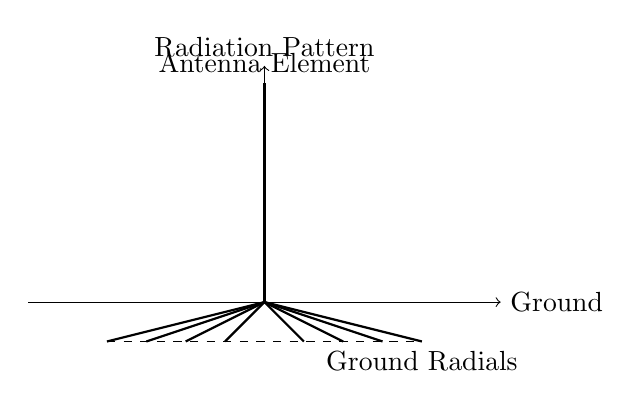
\begin{tikzpicture}
    \draw[->] (-3,0) -- (3,0) node[right] {Ground};
    \draw[->] (0,0) -- (0,3) node[above] {Radiation Pattern};
    \draw[thick] (0,0) -- (0,2.78) node[above] {Antenna Element};
    \draw[dashed] (-2,-0.5) -- (2,-0.5) node[below] {Ground Radials};
    \foreach \x in {-2,-1.5,-1,-0.5,0.5,1,1.5,2} {
        \draw[thick] (0,0) -- (\x,-0.5);
    }
\end{tikzpicture}
\end{center}
